  
  O Protégé é uma ferramenta que permite a construção de ontologias de domínio, como também, a personalização de formulários
  de entrada de dados e inserção e edição de dados,  possibilitando assim, a criação de bases de conhecimento guiadas por ontologias.
  \cite{semprebom07}
  
  Para a construção da ontologia deste projeto, foi utilizada a versão (3.1) do Protégé. A Figura \ref{fig:interface_protege} ilustra
  a interface gráfica da ferramenta, que prôve acesso a ferramentas e menus, além de cinco áreas de vizualização (\textit{views}) que 
  se comportam como módulos de navegação e edição de classes, atributos, formulários e instâncias, propiciando entrada de dados,
  recuperação das informações e pesquisas na base de conhecimento. \cite{semprebom07}
  
  \begin{figure}[h] 
    \centering 
    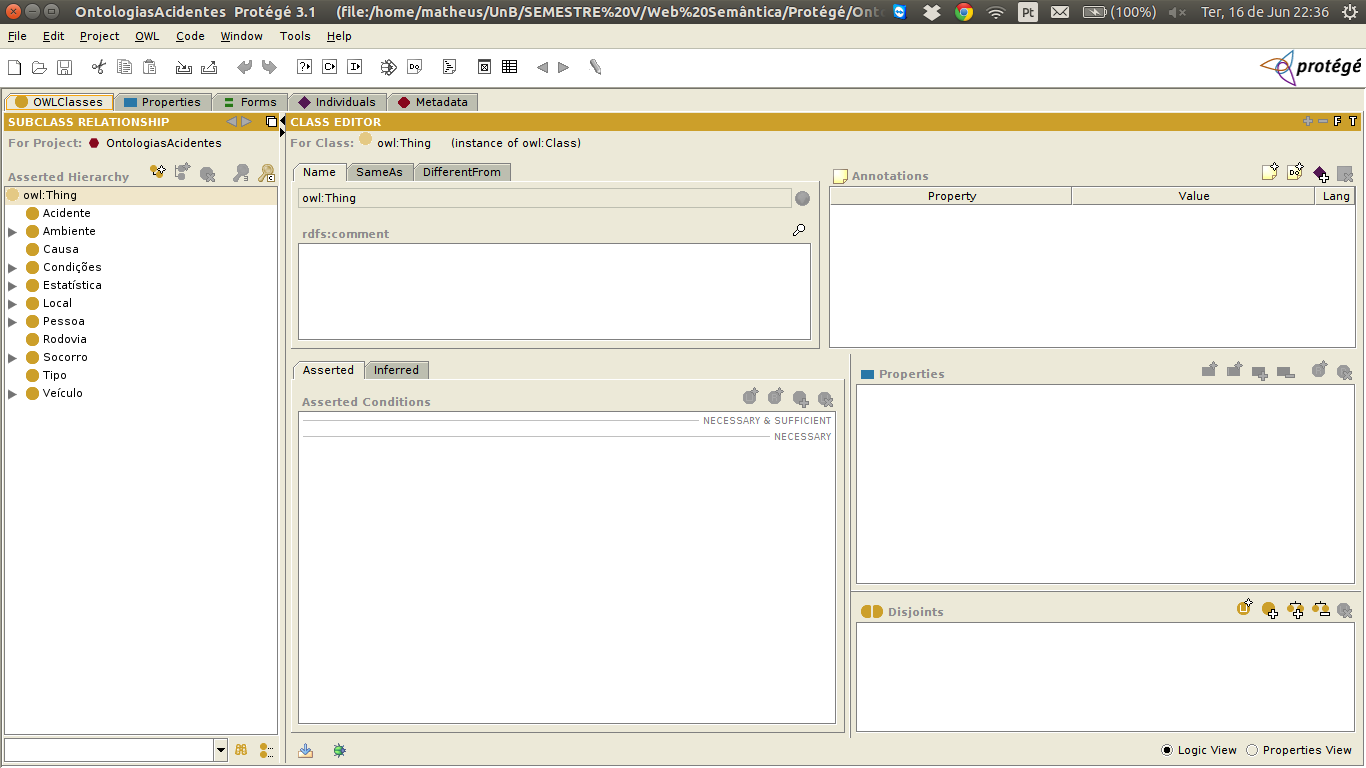
\includegraphics[scale=0.3]{interface_protege} 
    \caption[Interface gráfica do Protégé]
    {Interface gráfica do Protégé}
    \label{fig:interface_protege}
  \end{figure}
  
\subsection{Características do Protégé}

  Esta seção apresenta algumas características da ferramenta Protégé que estão listadas abaixo: 
  (\citeauthor{semprebom07}, \citeyear{semprebom07} \textit{apud} \citeauthor{freitas04}, \citeyear{freitas04}).
  
  \begin{itemize}
    \item A linguagem PAL (\textit{Protégé Axiomatic Language}, uma linguagem axiomática, permite a inserção de restrições e axiomas
    que incidem sobre classes e instâncias pertencentes a uma ou mais ontologias;
    \item A ferramenta provê a geração de arquivos de saída alteráveis, onde podem ser criadas classes e instâncias em CLIPS (motor 
    de inferência) - a base de conhecimento é gerada nativamente para esse motor.
    \item Interface para entrada de conhecimento, com um gerador automático de formulários para classes definidas. A reposição da interface
    original por componentes mais adequados à aplicação é admitida. A interface da ferramenta facilita, sobretudo, o gerenciamento de
    conhecimento de uma ou mais ontologias.    
  \end{itemize} 
  
      Os arquivos de saída suportados são: Jess, F-Logic, Prolog, RDF, OIL, XML, Topic Maps. \cite{semprebom07}